\graphicspath{{content/chapters/7_evaluation/figures/}}
\chapter{Evaluation}
\label{chp:evaluation}

This chapter presents a comprehensive evaluation of the implemented speech enhancement system, assessing both classical and deep learning approaches across several dimensions. The evaluation is divided into three key parts. First, the impact of dataset handling strategies is examined, comparing how the different dataset methods affect training efficiency and performance. Second, the effectiveness of Out-of-Memory (OOM) mitigation techniques is validated to ensure that memory-saving strategies do not degrade model quality. Finally, the core focus of this chapter is a comparative analysis of model architectures, benchmarking five machine learning models against three classical denoising methods.

Each section includes detailed quantitative assessments using respective metrics. The metrics within the first three sections are conducted in batch. That is the model is trained on the whole training set, the validation on the whole validation set, and the denoising on the whole test set. So any metrics are averaged across the whole dataset. Results are presented using clear, tabulated formats for ease of interpretation and cross-comparison.

\section{Dataset Performance}
\label{sec:dataset_performance}

This section examines the performance of the three dataset handling strategies: Static Bucketing, Dynamic Bucketing, and Padding-Truncation Output-Truncation (PTO). The goal is to assess how these strategies affect the overall efficiency of the training process, particularly in terms of dataset loading times, runtime overhead during training, and their influence on model performance. Each strategy was tested using the same model architecture, the Contextual Encoder-Decoder (CED), chosen for its simplicity and effectiveness in the spectrogram domain. Under two conditions:

\begin{itemize}
    \item \textbf{Cold Run (Uncached):} In this scenario, all dataset operations are executed from scratch. Static and Dynamic Bucketing compute bucket assignments (with Dynamic Bucketing also requiring K-Means clustering), while PTO calculates and stores the original waveform lengths. This setup simulates a first-time deployment or training on a fresh system.
    
    \item \textbf{Warm Run (Cached):} This run utilizes cached data generated during the cold run, significantly reducing load and preprocessing time. For Static and Dynamic Bucketing, bucket mappings and K-Means centers are reloaded. For PTO, the previously computed original sequence lengths are retrieved.
\end{itemize}

The configuration used for all CED runs is shown in Figure~\ref{fig:dataset_config}, with the only varying parameter being the \texttt{PAD\_METHOD}.

\begin{figure}[H]
    \centering
    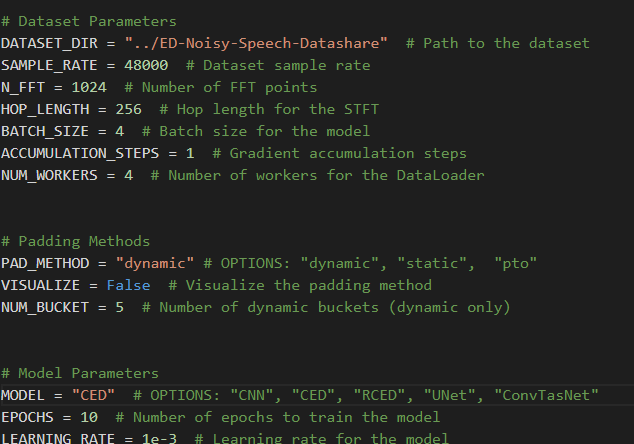
\includegraphics[width=0.8\textwidth]{dataset_config.png}
    \caption{\label{fig:dataset_config} Configuration of the CED model used for dataset performance evaluation.}
\end{figure}

Both uncached and cached runs were executed, and the relevant timing metrics were collected from the output logs, as shown in Table~\ref{tab:dataset_loading_times}.

\vspace{1em}
\begin{table}[H]
\centering
\caption{Dataset Training Overheads}
\label{tab:dataset_loading_times}
\begin{tabular}{|l|c|c|c|}
\hline
\textbf{Dataset} & \textbf{Uncached} & \textbf{Cached} & \textbf{Truncation Overhead} \\
\hline
Static Bucketing  & 296.85s  & 0.83s   & N/A    \\
Dynamic Bucketing & 581.57s& 0.83s  & N/A    \\
PTO               & 288.47s & 0.79s  & 68.62s  \\
\hline
\end{tabular}
\end{table}

The results in Table~\ref{tab:dataset_loading_times} reveal key insights into the efficiency of each dataset handling strategy. In the uncached condition, both Static Bucketing and PTO exhibit similar loading times, as each only requires a single pass through the dataset. Either to assign buckets or compute original waveform lengths. Dynamic Bucketing, however, incurs nearly double the loading time due to the additional K-Means clustering step, which requires a second pass to calculate cluster centers for optimal bucket assignment. This overhead is particularly pronounced in the uncached scenario, where the dataset must be fully loaded and processed from scratch.

In contrast, the cached runs significantly reduce loading times across all methods. Once the dataset metadata has been computed and stored, subsequent runs simply reload the cached mappings or original lengths, avoiding repeated preprocessing. PTO achieves the fastest cached time, as retrieving a list of original lengths is marginally quicker than reloading bucket assignments or cluster centers. However, a key distinction of PTO is its requirement for per-epoch output truncation during training. While this truncation overhead is relatively minor compared to the total training duration (typically on the order of hours). It can accumulate significantly across large datasets or extended training schedules. This trade-off must be carefully considered when assessing PTO's suitability for time-sensitive or resource-constrained training environments.

To evaluate the impact of dataset handling strategies on model learning, each method was tested using the best-performing checkpoint from its respective training run. Since the differences in performance between cached and uncached conditions were found to be trivial, the results reported in Table~\ref{tab:dataset_performance} reflect the mean values across runs, with corresponding margins of error. This provides a clearer picture of any underlying variation while confirming the consistency of results.

\vspace{1em}
\begin{table}[H]
\centering
\caption{Dataset Handling Strategies Training Metrics}
\label{tab:dataset_performance}
\begin{tabular}{|l|c|c|c|}
\hline
\textbf{Dataset} & \textbf{Train Loss} & \textbf{Val Loss} & \textbf{Val SNR} \\
\hline
Static Bucketing  & \(0.1805 \pm 0.0013\)  & \(0.1787 \pm 0.0020\)  & \(0.54 \pm 0.045\) dB \\
Dynamic Bucketing & \(0.1779 \pm 0.0004\)  & \(0.1850 \pm 0.0063\)  & \(0.56 \pm 0.010\) dB \\
PTO               & \(0.1414 \pm 0.0019\)  & \(0.1458 \pm 0.0033\)  & \(0.53 \pm 0.050\) dB \\
\hline
\end{tabular}
\end{table}

The results in Table~\ref{tab:dataset_performance} show that while all three dataset handling strategies yield reasonable and consistent validation SNR values, there are notable differences in training and validation loss. In particular, the PTO method achieves lower training and validation loss compared to both Static and Dynamic Bucketing. This suggests that PTO facilitates more learning under the current loss formulation.

However, despite its lower loss, PTO does not yield a corresponding improvement in validation SNR. The SNR values across all methods remain within a narrow range, indicating that the perceptual or energy-based denoising quality is comparable. The improved loss values in PTO may be partly influenced by its output truncation mechanism. This evaluates only the central, non-padded regions of the spectrogram. Potentially leading to more favorable loss estimates even if the actual perceptual improvement is marginal.

Considering the trade-offs between implementation complexity, runtime overhead, and generality. Dynamic Bucketing remains the most balanced choice. It handles variable-length inputs with optimal bukceting and minimal padding. Avoids the per-epoch truncation overhead of PTO and maintains reliable performance across all metrics. As such, Dynamic Bucketing is selected as the preferred dataset handling strategy for all subsequent model evaluations in this project.

\section{OOM Validation}
\label{sec:oom_validation}

While Section~\ref{sec:oom_handling} outlined several techniques to mitigate Out-of-Memory (OOM) errors during training. It is important to demonstrate that these strategies do not compromise model learning. The goal of this section is to validate that memory-saving methods do not lead to information loss or degraded performance. To assess this, the RCED model was used, since the UNet and ConvTasNet could not be trained without OOM-handling techniques. Training was conducted using the dynamic bucketing strategy and compared across three different configurations:

\begin{enumerate}
    \item \textbf{Clean Training (Control):} A standard training loop without any OOM-handling logic, using a batch size of 4. This configuration serves as the control, with no memory management mechanisms.
    
    \item \textbf{OOM Handling (Batch 4, Accum 1):} OOM-handling techniques were enabled while maintaining a batch size of 4. These included fixed-point precision (FP16) and garbage collection (GC), allowing for a more memory-efficient training process.
    
    \item \textbf{OOM + Accumulation (Batch 2, Accum 2):} The batch size was reduced to 2, with gradient accumulation set to 2, simulating an effective batch size of 4. All OOM-handling techniques remained enabled. This configuration is designed to reduce memory usage while preserving gradient stability.
\end{enumerate}

Each configuration was trained for the same number of epochs, using identical learning rates and optimizers. Table~\ref{tab:oom_training} summarizes the training and validation performance.

\vspace{1em}
\begin{table}[H]
\centering
\caption{OOM Configurations Training Metrics}
\label{tab:oom_training}
\begin{tabular}{|l|c|c|c|c|}
\hline
\textbf{Train Config} & \textbf{Train Loss} & \textbf{Val Loss} & \textbf{Val SNR} & \textbf{Training Time} \\
\hline
Control                & 0.1169 & 0.1185 & 3.20 dB & 4.44 h \\
OOM Handling           & 0.1217 & 0.1255 & 2.74 dB & 3.08 h \\
OOM + Accumulation     & 0.1184 & 0.1263 & 2.95 dB & 3.91 h \\
\hline
\end{tabular}
\end{table}

The results in Table~\ref{tab:oom_training} show that all three training configurations achieve comparable performance in terms of both loss and validation SNR. The control configuration, which does not use any OOM-handling mechanisms, achieves the best validation SNR of 3.20 dB. With the differences across configurations being within a 0.5 dB range. Suggesting that the inclusion of OOM-handling strategies does include some degradation of the models training performance. The OOM Handling configurations, use of FP16 and GC could be seen as a trade-off between memory efficiency and model performance. 

Each configuration was further evaluated in the full denoising pipeline. Table~\ref{tab:oom_metrics} presents the performance metrics across key evaluation criteria.

\vspace{1em}
\begin{table}[H]
\centering
\caption{OOM Configurations Denoising Metrics}
\label{tab:oom_metrics}
\begin{tabular}{|l|c|c|c|c|c|}
\hline
\textbf{Train Config} & \textbf{↑SNR} & \textbf{↓MSE} & \textbf{↑PESQ} & \textbf{↑STOI} & \textbf{↓LSD} \\
\hline
Control              &  14.2843 & 0.000120 & 2.1096 & 0.8730 & 0.702311 \\
OOM Handling           & 14.7731 & 0.000114 & 2.1791 & 0.8783 & 0.691936 \\
OOM + Accumulation     & 14.8076 & 0.000117 & 2.1008 & 0.8748 & 0.692152 \\
\hline
\end{tabular}
\end{table}

The results in Table~\ref{tab:oom_metrics} reveal that, contrary to initial expectations, the OOM-handling configurations not only maintain performance but slightly outperform the control in several key denoising metrics. Both the \textbf{OOM Handling} and \textbf{OOM + Accumulation} setups show improvements in SNR, PESQ, and LSD, suggesting enhanced perceptual quality and spectral fidelity.

Specifically, \textbf{OOM + Accumulation} achieves the highest SNR at 14.81 dB, marginally outperforming both the control and the non-accumulated OOM variant. Additionally, the lowest LSD values are observed in the OOM-handled models, indicating that their outputs more closely preserve the spectral characteristics of the clean reference signals. These findings suggest that the use of FP16 precision and memory-aware strategies does not harm. Potentially even improving the model's ability to generalize. 

The marginal gains in PESQ and STOI further support this conclusion. Although the differences are subtle, they point to a stable perceptual consistency across configurations. It is also possible that reduced numerical precision in FP16 introduces a form of implicit regularization, slightly mitigating overfitting and improving generalization performance.

In summary, while the training metrics in Table~\ref{tab:oom_training} showed modest differences across configurations. The downstream denoising evaluation shows no degradation and in some cases minor improvements. These findings fully justify the use of OOM-handling techniques throughout this project. Even if future configurations exhibited performance regressions due to OOM mitigation. Their use would remain essential for enabling the training of memory-intensive models such as \textit{UNet} and \textit{Conv-TasNet}, ensuring a fair architectural comparison across all model types evaluated in this work.

\section{Model Performance}
\label{sec:model_performance}

This section presents the most critical part of the evaluation and the central focus of the project. A comparative assessment of classical methods and five machine learning models for speech enhancement. Unlike earlier evaluations, which focused on dataset handling strategies and OOM mitigation techniques using fixed models to conduct the justification. The main scope of this project is to justify the use of machine learning models for speech enhancement and to evaluate their performance against classical methods.

The evaluation retains the previously established dynamic bucketing and OOM-handling strategies to ensure consistency. To provide a meaningful frame of reference, a baseline set of metrics is also established in Section~\ref{sec:classical_methods}. This baseline follows the same evaluation pipeline as the classical methods but uses the raw noisy inputs directly compared against the clean reference signals. These values define a lower bound for performance and serve as a clear reference point for assessing the effectiveness of each denoising method.

\subsection{Classical Methods}
\label{sec:classical_methods}

The classical methods evaluated include Spectral Subtraction (SS), Wiener Filtering (WF), and the Minimum Mean Square Error - Log Spectral Amplitude estimator (MMSE-LSA).These are all implemented in a single-channel setting. SS and WF are foundational methods in literature, whilst MMSE-LSA represents a more developed and perceptually motivated approach. Since these methods do not require training, the classical evaluation focuses solely on denoising performance using the same pipeline and evaluation metrics as the learning-based models.

\vspace{1em}
\begin{table}[H]
\centering
\caption{Classical Denoised Metrics}
\label{tab:classical_metrics}
\begin{tabular}{|l|c|c|c|c|c|c|}
\hline
\textbf{Method} & \textbf{↑SNR} & \textbf{↓MSE} & \textbf{↑PESQ} & \textbf{↑STOI} & \textbf{↓LSD} & \textbf{Denoise Time} \\
\hline
Baseline     & -2.2774 & 0.005152 & 1.8451 & 0.8928 & 0.904223 & 56s \\
SS          & 3.0861 & 0.001525 & 1.4535 & 0.8457 & 0.767089 & 1.01 m \\
WF          & 0.4647 & 0.002875 & 2.0639 & 0.8889 & 0.753452 & 1.21 m \\
MMSE-LSA    & -0.8619 & 0.003726 & 2.0238 & 0.8943 & 0.797070 & 1.39 m \\
\hline
\end{tabular}
\end{table}

The results in Table~\ref{tab:classical_metrics} highlight the differing trade-offs established by each classical denoising method. Importantly, the inclusion of baseline metrics provides a critical point of reference for evaluating both classical and learning-based models. Without it, the negative SNR value for MMSE-LSA would misleadingly suggest a failure in denoising—when in fact, it still reduces noise energy effectively.

SS achieves the best improvement in SNR and MSE, reflecting strong numerical suppression of noise. However, this comes at the cost of perceptual quality, as evidenced by its relatively low PESQ and STOI scores. This is likely due to spectral over-subtraction and residual artifacts, which degrade perceived audio quality.

In contrast, WF and MMSE-LSA adopt more perceptually driven strategies. WF achieves the best PESQ (2.0639) and the lowest LSD (0.753), indicating better preservation of spectral fidelity. Its performance benefited from an adjustment in noise estimation. Where the noise PSD was computed using the mean of the first six STFT frames rather than the minimum—resulting in more stable and effective filtering. MMSE-LSA records the highest STOI (0.8943), suggesting superior intelligibility of speech content. While iterative tuning helped stabilize its behavior, MMSE-LSA inherently prioritizes log-spectral distortion minimization. As a result, it achieves clear perceptual improvements but offers less numerical gain in SNR compared to SS or WF. This trade-off is consistent with its design focus on perceptual quality over raw energy preservation.

The negative SNR values for both the baseline and MMSE-LSA arise primarily from averaging across test files with highly variable and often low input SNRs. In such cases, even minor reconstruction errors can dominate energy calculations, pulling the average SNR below zero—despite the clear perceptual improvements reflected in PESQ and STOI.

All classical methods complete denoising in under two minutes, confirming their practicality for batch processing and their suitability for real-time deployment when computational efficiency is essential.

\subsection{Machine Learning Models}
\label{sec:ml_models}

\subsubsection{Training Metrics}
\label{sec:training_metrics}

With the classical methods evaluated, the focus now shifts to the machine learning models. Each model defined in the \ref{sec:model_architecture} section was trained using the same dataset handling strategies and OOM mitigation techniques previously established. The models followed a consistent training configuration: a batch size of 2, accumulation steps of 4, 25 training epochs, and a learning rate of $1 \times e^{-3}$. The table below summarizes the training performance for each model.

\vspace{1em}
\begin{table}[H]
\centering
\caption{Machine Learning Models Training Metrics}
\label{tab:ml_training}
\begin{tabular}{|l|c|c|c|c|}
\hline
\textbf{Model} & \textbf{Train Loss} & \textbf{Val Loss} & \textbf{Val SNR} & \textbf{Training Time} \\
\hline
CNN         & 0.2855 & 0.4292 & 0.45 dB & 4.01 h \\
CED         & 0.1599 & 0.1675 & 0.88 dB & 6.32 h \\
RCED        & 0.1136 & 0.1239 & 2.69 dB & 7.43 h \\
UNet        & 0.0477 & 0.0649 & 6.35 dB & 17.44 h \\
ConvTasNet  & 0.0438 & 0.0478 & 9.23 dB & 1d 1.25h \\
\hline
\end{tabular}
\end{table}

The training outcomes summarized in Table~\ref{tab:ml_training} clearly demonstrate a consistently increamenting trend in performance as the models progress in complexity. 

The CNN model was introduced as a simple foundation to validate the project’s training and evaluation pipeline. It demonstrated reasonable training metrics, though not directly comparable to the classical methods, which do not involve a learning phase. The training plot in Figure~\ref{fig:cnn_training_plot} shows a moderate gap between training (0.2855) and validation (0.4292) loss, around a 50\% increase indicating moderate overfitting. Additionally, the validation loss increases during the early epochs, likely due to the model initially overfitting to noise patterns in the training data before learning more generalizable features. Despite this, the validation SNR continues to improve steadily, suggesting that the model gradually captures meaningful structure in the data.

\begin{figure}[H]
    \centering
    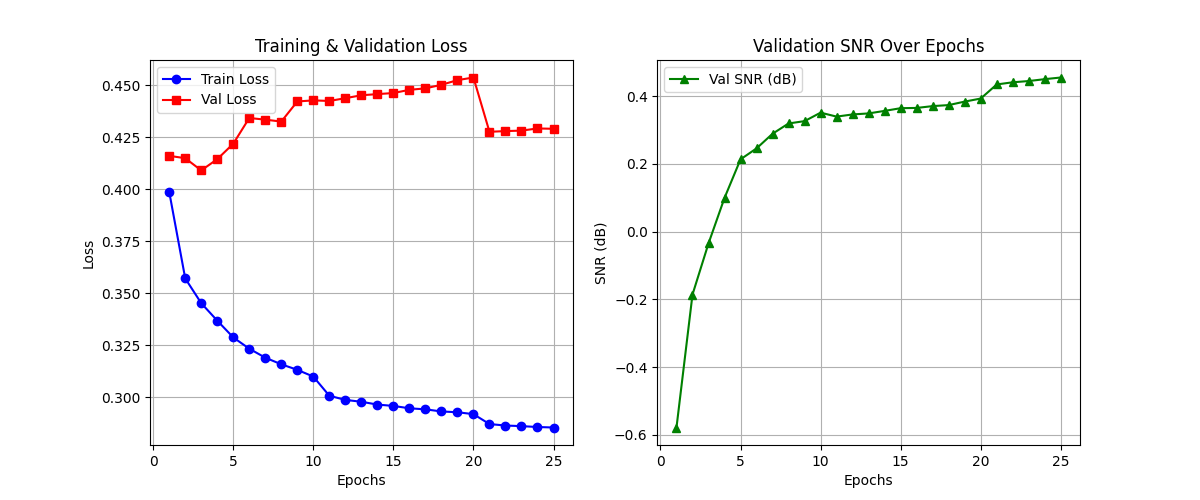
\includegraphics[width=0.8\textwidth]{CNN_plot.png}
    \caption{\label{fig:cnn_training_plot} CNN training plot.}
\end{figure}

The CED model expands upon the CNN baseline by adopting a fully connected encoder-decoder architecture. It delivers significant performance gains for only a modest increase in model complexity and training time. As shown in Figure~\ref{fig:ced_training_plot}, both the training and validation loss curves converge smoothly and remain closely aligned throughout training, indicating stable learning and minimal overfitting.

\begin{figure}[H]
    \centering
    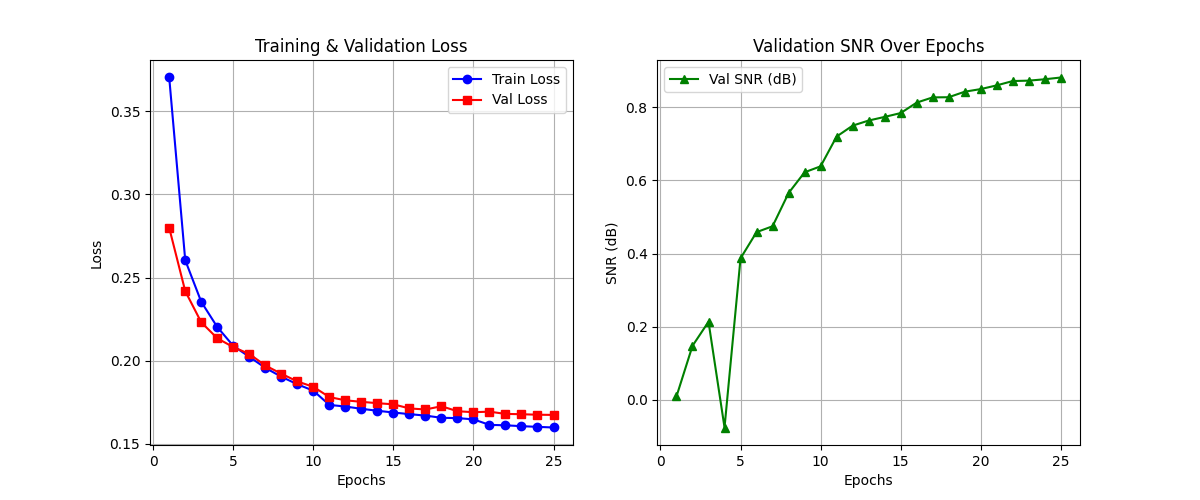
\includegraphics[width=0.8\textwidth]{CED_plot.png}
    \caption{\label{fig:ced_training_plot} CED training plot.}
\end{figure}

The RCED model extends the CED architecture by incorporating residual connections to improve information flow and gradient propagation. As shown in Table~\ref{tab:ml_training}, RCED outperforms CED across all training metrics, with validation SNR increasing from 0.88 dB to 2.69 dB and only a minor increase in training time.

The training plot in Figure~\ref{fig:rced_training_plot} shows stable convergence in loss curves, though the validation SNR exhibits more fluctuation compared to CED. These oscillations likely stem from the model’s increased sensitivity due to its added complexity with residual connections. Nevertheless, the upward SNR trend confirms that RCED generalizes effectively and benefits from residual learning. Supporting the findings of \cite{park2017acoustic}.

\begin{figure}[H]
    \centering
    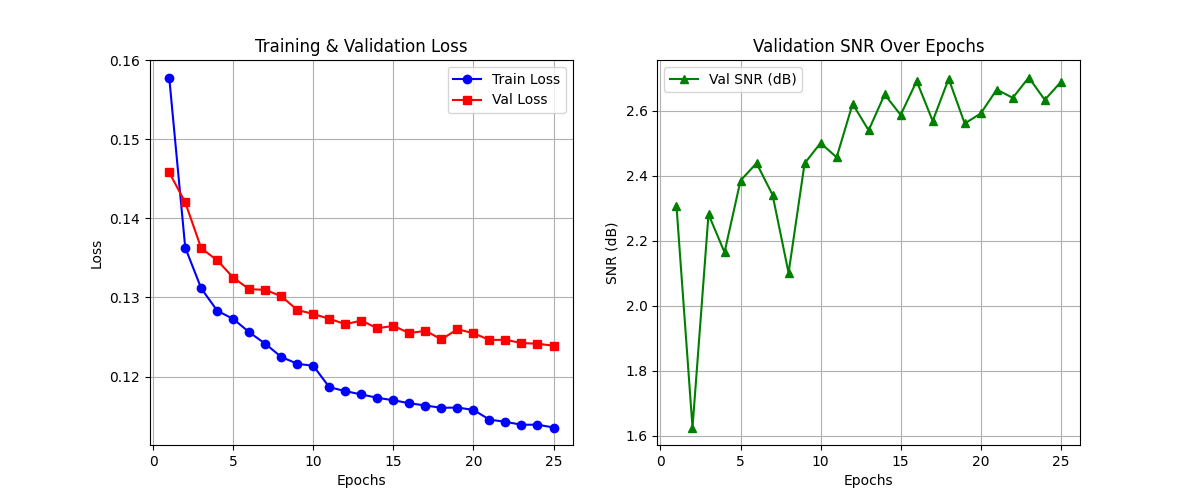
\includegraphics[width=0.8\textwidth]{RCED_plot.png}
    \caption{\label{fig:rced_training_plot} RCED training plot.}
\end{figure}

The UNet model achieved the best training and validation loss so far, with loss values of 0.0477 and 0.0649 respectively, and more than doubled the validation SNR to 6.35 dB compared to RCED. This reflects the strength of its skip connected encoder-decoder architecture, which helps preserve fine grained spectral details during reconstruction.

However, this performance comes at a significant cost. UNet required 17.44 hours to train, over twice the duration of RCED. As shown in Figure~\ref{fig:unet_training_plot}, the model converges smoothly, and the validation SNR shows a consistent upward trend with fewer fluctuations than RCED. It is worth noting that all recorded training times are situational and can vary with configuration and system load. A full justification of these time performance trade offs is provided in Section~\ref{sec:denoising_metrics}.

\begin{figure}[H]
    \centering
    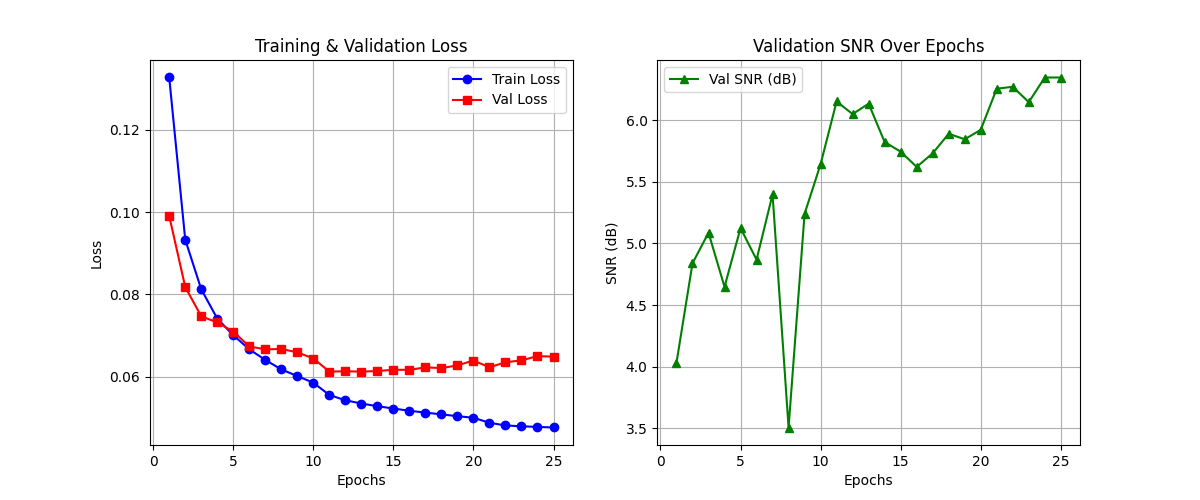
\includegraphics[width=0.8\textwidth]{UNet_plot.png}
    \caption{\label{fig:unet_training_plot} UNet training plot.}
\end{figure}

The ConvTasNet model yielded the most notable training results. It achieved the lowest loss values 0.0438 (train) and 0.0478 (validation). The highest validation SNR of 9.23 dB, a substantial improvement over UNet’s 6.35 dB. As shown in Figure~\ref{fig:convtasnet_training_plot}, the model demonstrates strong convergence, with the validation SNR stabilizing at a high level after initially fluctuating. This behavior reflects ConvTasNet’s ability to model complex temporal dependencies more effectively than the previous architectures.

However, this performance came at a computational cost. ConvTasNet required over 25 hours to train, marking the longest training time in this project. This trend of increasing training duration aligns with the growing complexity and capacity of the models. As architectures become more expressive, it becomes harder to extract further improvements in SNR, necessitating longer optimization cycles to refine smaller, higher level features.

\begin{figure}[H]
    \centering
    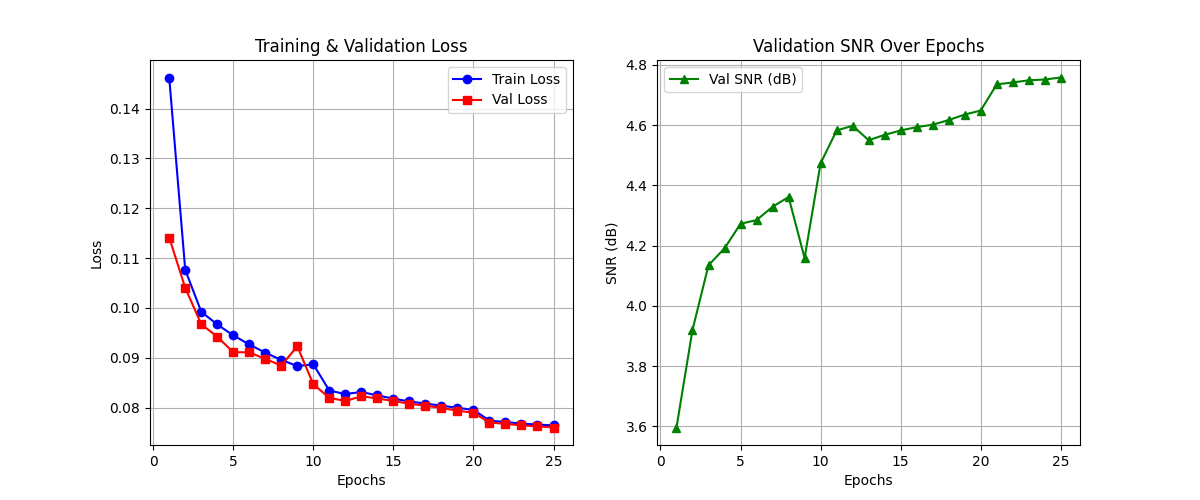
\includegraphics[width=0.8\textwidth]{ConvTasNet_plot.png}
    \caption{\label{fig:convtasnet_training_plot} ConvTasNet training plot.}
\end{figure}

In summary, the training phase across all models showed a clear upward trend in learning capacity and output quality. Each architectural refinement from CNN to ConvTasNet yielded measurable improvements in loss and SNR, though at the expense of increased training time and complexity. This trade off sets the stage for a comprehensive evaluation in the next section, where these models are benchmarked on real denoising performance.

\subsubsection{Denoising Metrics}
\label{sec:denoising_metrics}

Following the training phase, each machine learning model was evaluated using the same denoising pipeline and metrics applied to the classical methods. The results in Table~\ref{tab:ml_denoise} summarize performance across objective and perceptual criteria. Consistent with the training phase, the evaluation reveals the same trend of increasing model complexity correlating to improved denoising quality.

\vspace{1em}
\begin{table}[H]
\centering
\caption{Machine Learning Denoising Metrics}
\label{tab:ml_denoise}
\begin{tabular}{|l|c|c|c|c|c|c|}
\hline
\textbf{Model} & \textbf{↑SNR} & \textbf{↓MSE} & \textbf{↑PESQ} & \textbf{↑STOI} & \textbf{↓LSD} & \textbf{Denoise Time} \\
\hline
CNN         & 4.6432  & 0.001344 & 1.7410 & 0.8073 & 0.795551 & 1.11 m \\
CED         & 13.1850  & 0.000161 & 1.6780 & 0.8386 & 0.765542 & 1.05 m \\
RCED        & 14.5285  & 0.000117 & 2.0542 & 0.8677 & 0.647985 & 1.14 m \\
UNet        & 16.9872  & 0.000069 & 2.1384 & 0.8940 & 0.707572 & 1.27 m \\
ConvTasNet  & 18.0607 & 0.000063 & 2.4329 & 0.9112 & 0.674051 & 2.19 m \\
\hline
\end{tabular}
\end{table}

The CNN model, although introduced as a simple foundation, already outperforms all classical methods in numerical metrics. It achieves an SNR of 4.64 dB and an MSE of 0.001344, improving on SS’s 3.08 dB and 0.001525, respectively. However, it underperforms in perceptual quality, with a PESQ of 1.74 and STOI of 0.81, falling short of both WF and MMSE-LSA. This suggests that while the CNN effectively suppresses noise energy, its simple architecture distorts perceptual features. Its LSD of 0.80 confirms moderate fidelity to the original spectral structure but still shows room for improvement.

The introduction of the fully connected encoder-decoder architecture in CED presents a trade off between numerical and perceptual metrics. CED achieves slightly lower PESQ (1.68) and STOI (0.84) scores than CNN, indicating a perceptual quality drop, despite the design's intended purpose of improving it. However, the milestone in SNR (13.19 dB) and MSE (0.000161) are substantial enough to outweigh this perceptual dip. This substantial improvement likely came from the fixed overfitting experienced in the CNN. Now that a large portion of the noise energy is successfully suppressed, the models that follow must focus on enhancing perceptual quality to surpass the classical methods comprehensively.

Here, the results from \cite{park2017acoustic} are confirmed one last time with the RCED model. It delivers comprehensive improvements across all metrics, most notably in perceptual quality. Achieving a PESQ of 2.05 and a STOI of 0.87, values nearly on par with those of WF and MMSE-LSA. These gains justify the use of RCED over CED, as the added residual connections lead to meaningful enhancements in both intelligibility and naturalness.

The UNet model and introduction of skip connections is known to come at significant computational cost. However, the results in Table~\ref{tab:ml_denoise} show that this complexity is justified by the model's performance. UNet achieves a significant SNR of 16.99 dB, a PESQ of 2.14, and a STOI of 0.89. This is the first model to pass all classical methods in all metrics. It’s important to note that the closer we get to the clean signal, the harder it is to improve the results.

Finally, we have the ConvTasNet model. The most complex design out of all the models and computationally expensive. ConvTasNet achieves remarkable results across all metrics, with an SNR of 18.06 dB, a PESQ of 2.43, and a STOI of 0.91. These metrics are surely suitable for deployment standards in a small scale scenario. The LSE of 0.67 shows how we have moved closer to the clean signal whilst maintaining a good spectral representation. Overall, our model evalution ends with ConvTasNet achieving the best performance across all metrics compared to both all the classical methods and the other machine learning models.

